\documentclass[10pt,a4paper]{article}
\usepackage[utf8]{inputenc}
\usepackage{amsmath}
\usepackage{amsfonts}
\usepackage{amssymb}
\usepackage{eucal}
\usepackage{physics}
\usepackage{graphicx}

\begin{document}

\section{Introduction}

Quantum computing has meant a paradigm shift in computer science, introducing a new era of computational power and possibilities. By leveraging the principles of quantum mechanics, quantum computing offers capabilities far beyond those of classical computers. Although quantum hardware is still evolving, Noisy Intermediate-Scale Quantum (NISQ) \cite{Preskill} computers have already begun to unveil the potential of quantum computing, igniting widespread interest in implementing quantum algorithms that promise significant speedups over classical counterparts. In particular, the speedup of solving NP-complete problems is an area that quantum computing can tackle. In this paper, we have focused on the Hamiltonian Cycle Problem.\\
This problem is one of Karp's 21 seminal NP-complete problems, it involves determining whether a given graph contains a Hamiltonian cycle—a cycle that visits every vertex exactly once. The problem is significant because of its similarities with the TSP, and its applications span various domains, including logistics and network optimization, where identifying optimal cycles is crucial AGREGAR CITAS. Traditional solution methods range from brute force approaches to sophisticated algorithms like dynamic programming and Monte Carlo simulations. In this paper, we propose utilizing Grover's algorithm to tackle the HC problem, offering the potential for quadratic speedup.\\
The structure of this paper is as follows. An explanation of Grover's algorithm is given in Section II. The proposed methodology is given in Section III. Section IV explores the existing solutions for the problem and compares the theoretical results.


\section{Background}
\subsection{Grover's Algorithm}

The search algorithm developed by Lov K. Grover in 1997 \cite{Grover1} is a milestone in the development of quantum algorithms. It solves the problem of finding a tagged element (or $M$ elements) in a disordered set of $N$ elements using $k_{Gr}= \lfloor\frac{\pi}{4} \sqrt{\frac{N}{M}}\rfloor$ times a system, called oracle, which is able to identify this element. It presents a quadratic improvement in order relative to the classical brute-force search algorithm, which requires in the worst-case scenario N system calls. Grover's algorithm does not converge with 100\% probability to the desired state, it converges with an arbitrarily high probability that depends on the relationship between solutions and the size of the search space.\\
As Grover proposed later, the algorithm can be used to speed up the solution of NP-complete problems \cite{Grover2}. Since, its application has been explored with some problems such as Clique problem \cite{Clique, Clique2}, k-coloring \cite{Coloring1, Coloring2} and SAT \cite{SAT_ions, SAT_paralel}. Nielsen and Chuang predicted the solution of the HC problem using Grover\cite{Nielsen_Chuang_2010}.\\
The original problem presented by Grover \cite{Grover1} is as follows. Let there be a set of $N = 2^n$ quantum states in a Hilbert space ($\mathcal{H}_n$), where n is the number of qubits, and an unknown canonical basis state marked between them (solution to the problem). Given a system, an operator, called an oracle that identifies the marked element, the objective is to find this marked element with high probability, using as few queries to the oracle as possible.\\
Let $\ket{t}$ be the marked element of the base, and $\ket{s}$ the uniform superposition of all basis states. An oracle operator $O = I_d - 2\ket{t}\bra{t}$ is applied and changes the phase of the marked state. A diffusion operator $D = I_d - 2\ket{s}\bra{s}$ is applied and amplifies the amplitude of the marked state. Applying the Grover operator $(G=DO)$ $k_{Gr}$ times maximizes the probability of measuring $\ket{t}$.\\
A more detailed and extended explanation for when the set has more than one solution can be found in reference \cite{Nielsen_Chuang_2010}.

AGREGAR DIAGRAMA DE GROVER QUE ESTE LINDO.

\subsection{Hamiltonian Cycle Problem}
Explicamos qué es el Hamiltonian Cycle Problem.
Explicamos cuáles son los principales usos de resolver el HCP.
Consultamos las heurísticas actuales de resolución del HCP.

\section{Proposed Algorithm for Hamiltonian Cycle Problem}
In order to solve a NP-complete problem with Grover's algorithm, it is necessary to translate a decision problem into a search problem. First, every possible cycle is encoded into a binary code. Let $G=(V, E)$ be the input graph with $N$ vertices and $e$ edges. $V = (v_1, ..., v_N)$ For every vertex, $n = \lceil \log_2 N \rceil$ are used to indicate the position it occupies in the cycle.\\
\begin{figure}[hbtp]
\centering
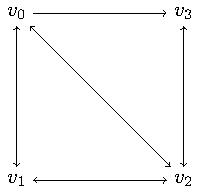
\includegraphics[scale=1]{figures/ExampleGraph.pdf}
\caption{Example Graph}
\end{figure}

For example the bitstring $11,00,01,10$ would be translated to $3-0-1-2$. This means $v_0$ is on the position $3$, $v_1$ in on the position $0$ and so on. The resulting cycle is $(v_1, v_2, v_3, v_0)$.
The search space includes every possible permutation of the positions of the vertices in the hamiltonian cycle. Therefore, its size is $2^{N\log n} = N^N$. The solutions of the HC problem satisfy two conditions:
\begin{enumerate}
\item Each vertex should have a different position.
\item Vertices with consecutive positions have to be connected by an edge. (The last and first positions are considered adjacent)
\end{enumerate}
\begin{table}[htbp]
    \centering
    \begin{tabular}{|c|c|c|c|}
        \hline
        Bitstring & Integer representation & Validity & Cycle \\
        \hline
        00,01,10,01 & 0-1-2-1 & Violates constraint 1 & None \\
        01,11,10,00 & 1-3-2-0 & Violates constraint 2 & $(v_3, v_0, v_2, v_1)$ \\
        00,11,10,01 & 0-3-2-1 & Yes & $(v_0, v_3, v_2, v_1)$\\
        \hline
    \end{tabular}
    \label{tab:example}
    \caption{Table with some examples of the solutions}
\end{table}

An algorithm to solve the HCP of a directed graph with $N = 2^n$ vertices is presented. The main contribution of this paper is the oracle $O$ that flips the phase of the states that satisfy both constraints. Later, possible adaptations of the algorithm for arbitrary graphs are proposed.

\subsection{Circuit definition}
The position index register $\ket{\psi}$, which covers the search space, has $m = N\log N$ qubits. Applying $O$ requires the addition of two registers, one for each constraint. An ancilla register $\ket{\theta}$ of $k = C^N_2$ qubits, and a second ancilla register $\ket{\zeta}$ with $l$ qubits. $l$ is the number of edges of the  complementary graph.

\subsection{Initialization}
Firstly, all position index qubits should be set in superposition of all states in the search space. This is done by applying the Hadamard Gate to each qubit in the main register. The qubits in the ancillas are set to $\ket{1}$ with the NOT gate. The resulting state is expressed as:
$$\ket{\psi_0} \otimes \ket{\theta_0} \otimes \ket{\zeta_0}$$
where:
$$\ket{\psi_0} = \frac{1}{\sqrt{2^m}}\sum_{i=0}^{m} \ket{i}$$
$$\ket{\theta_0} = \ket{1}^{\otimes k}$$
$$\ket{\zeta_0} = \ket{1}^{\otimes l}$$

\subsection{Oracle}

\subsubsection{Positional Exclusivity Block}
To satisfy the first constraint, the position of each vertex is compared with the position of every other vertex. The comparison is made by a comparator circuit defined in \cite{Coloring1}. The circuit, composed of NOT, CNOT and Toffoli/MCT gates, is applied to two registers of the same size, $a$ and $b$, and  stores the result in an ancilla qubit $o$.
$$\text{Comparator}(a, b, o) =
\begin{cases}
o \oplus 1, & \text{if } a = b; \\
o, & \text{if } a \neq b.
\end{cases}$$
\begin{figure}[hbtp]
\centering
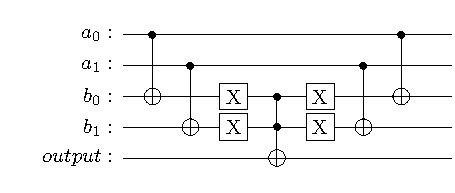
\includegraphics[scale=0.5]{figures/comparator.pdf}
\caption{Two bits Comparator circuit}
\end{figure}

The comparator circuit is applied to the $C^N_2$ combinations of position indexes, and each result is stored in a different qubit of $\ket{\theta}$ If any two vertices are assigned the same position, at least one qubit in $\ket{\theta}$ will be in state $\ket{0}$.

\begin{figure}[hbtp]
\centering
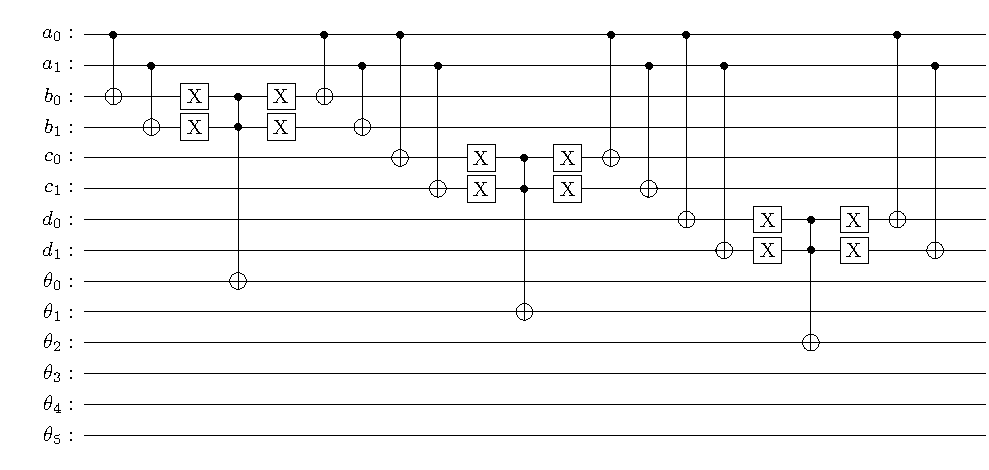
\includegraphics[scale=0.5]{figures/comparator_extended.pdf}
\caption{First three comparisons in the Positional Exclusivity block}
\end{figure}

\subsubsection{Missing Edge Detector Block}

Another subcircuit is introduced in this part, called the Plus One circuit. This circuit takes state $\ket{i}$ to state $\ket{(i+1) \mod 2^p}$. Given a register $q$ with $p$ qubits, a MCT is applied with the $p-1$ least significant qubits as control, and the most significant qubit as the target. This process is repeated taking with the $p-1$ least significant bits, so that every step the MCT has one less control. The inverse circuit, named Minus One circuit, takes state $\ket{i}$ to state $\ket{(i-1) \mod 2^p}$.
\begin{figure}[hbtp]
\centering
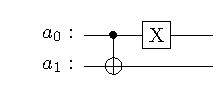
\includegraphics[scale=1]{figures/plus_one.pdf}
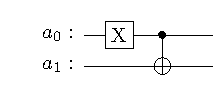
\includegraphics[scale=1]{figures/minus_one.pdf}
\caption{2 qubits Plus One circuit and Minus One Circuit}
\end{figure}

The missing edges set is defined as the set of edges of the complementary graph. In the example, the set of missing edges is $\{(1,3),(3,1),(3,0)\}$. To satisfy the second constraint, the vertices on adjacent positions should not have a missing edge between them.\\
The Plus One circuit is used to take the vertex to the next position, and then the Comparator circuit is used on the vertexes of the missing edge. If the next position of the vertex is occupied by a vertex that has a missing edge between them, the Comparator will flip an ancilla qubit.
\begin{figure}[hbtp]
\centering
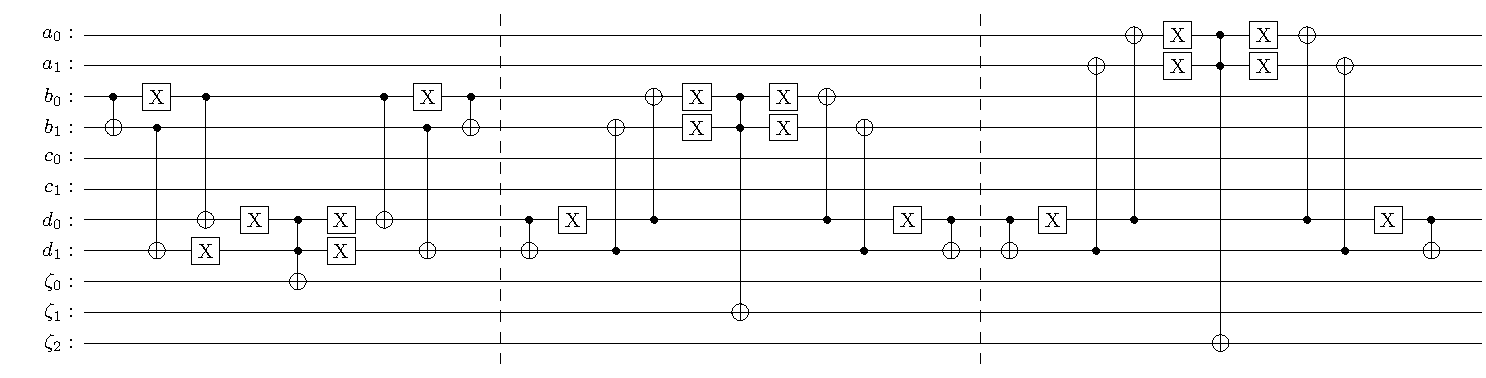
\includegraphics[scale=0.5]{figures/missing_edge.pdf}
\caption{Missing Edge block of the example above}
\end{figure}

\subsubsection{Complete Oracle Structure}
The complete oracle consists of the Positional Exclusivity Block, a Missing Edge Block, and a multi-controlled phase shift, acting in all the ancilla qubits. Then, the Positional Exclusivity Block and the Missing Edge Block are repeated to return the ancillas to their original state.

INSERTAR IMAGEN DE TODO EL ORACULO

\section{Generalization for an arbitrary graph}



\section{Informacion relevante para el futuro}


\bibliography{references.bib} 
\bibliographystyle{ieeetr}

\end{document}